In previous studies of the \WW\ final state the \dytt\ contribution
was considered small and well reproduced by the simulation since this
final state has a natural source of \met\ - neutrinos from $\tau$
decays. The fact that \met\ tends to be alligned with one of the
leptons is explored in the projected \met\ variable definition to
reduce the background rate.

With a rapid increase in the number of multiple interactions per bunch
crossing in 2011 data the situation is changing. Large amount of
pileup may lead to fake \met\ that is larger than the natural \met\
in \dytt\ events. Given that the \dytt\ cross-section is large and the
fact that we use a lower \met\ threshold in \emu\ final state we need
to make sure that this background is under control and reliably
estimated. Since the simulations that we have at the moment do not
reproduce the fake \met\ observed in data, we need a data-driven
method for the \dytt\ background estimation.

In order to estimate the \dytt\ background from data we can use \zee\
and \zmm\ events replacing electrons and muons with a simulated
$\tau\to l\nu_\tau\bar{\nu_e}$ decay - final state leptons will
represent the dilepton pair and neutrinos will modify obseved \met{}.

The simulation accounts for the $\tau$ decay polarization effects:
neglecting masses of electron, muon and neutrinos the angular
distribution of electron or muon originating from $\tau$ decay in
$\tau$ rest frame is
\begin{equation}
        \frac{d^2\Gamma}{dx\,d\cos\theta}\sim x^2(3-2x \pm P\cos\theta(2x-1))
\end{equation}
where $\theta$ is the helicity angle, i.e. angle between $\tau$ and
lepton direction in $\tau$ rest frame, $x=2E_l/m_\tau$ - reduced
energy, i.e. the energy of the lepton over its maximum allowed energy
and $P$ is degree of $\tau$ polarization~\cite{pdg}.

Figure~\ref{fig:dytt_closure} shows a comparison of some kinematic
distributions of \dytt\ Monte Carlo and a prediction based on \dymm\
Monte Carlo events using the procedure described above.

%% %%%%%%%%%%%%%%%%%%%%%%%%%%%%%%
%% \begin{figure}[!htbp]
%% \begin{center}
%% 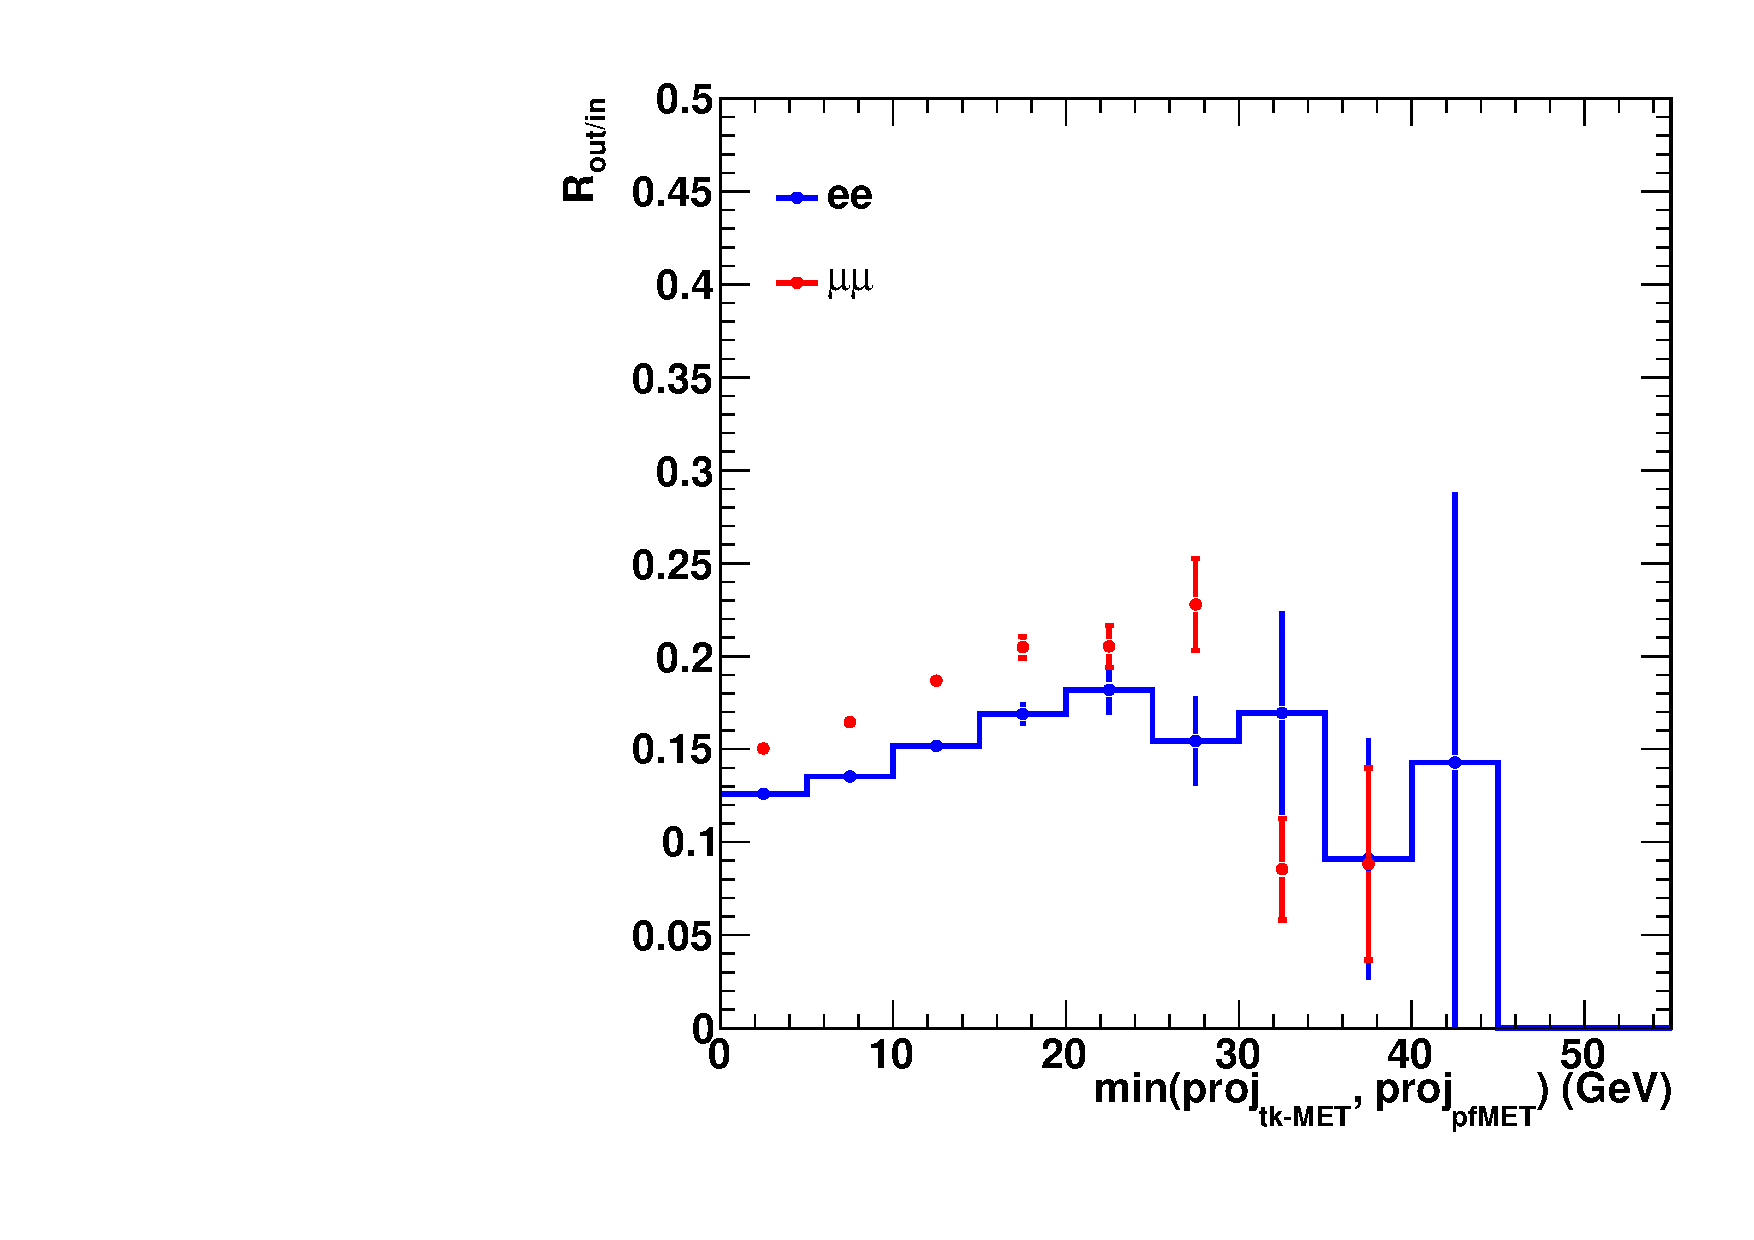
\includegraphics[width=0.3\textwidth]{figures/Routin_mc_0Jet.pdf}
%% 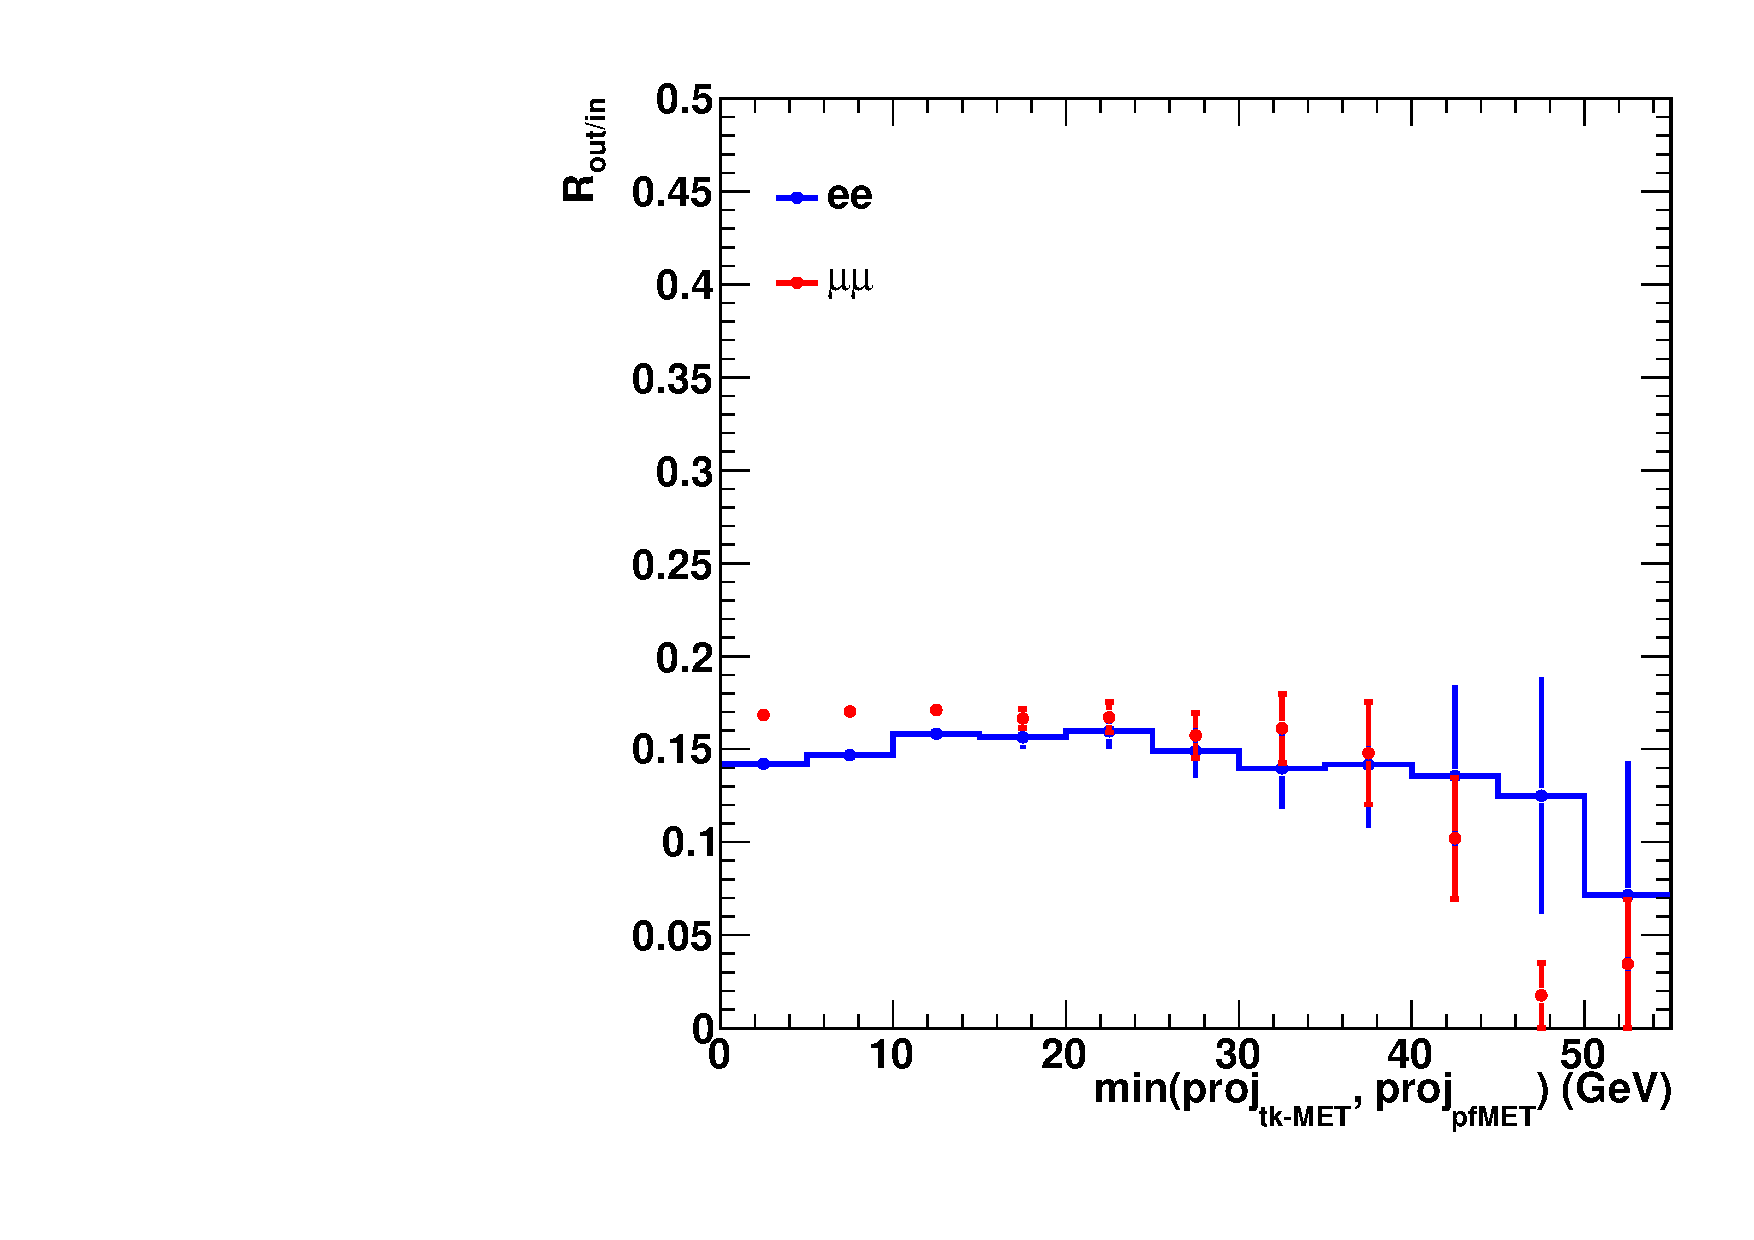
\includegraphics[width=0.3\textwidth]{figures/Routin_mc_1Jet.pdf}
%% 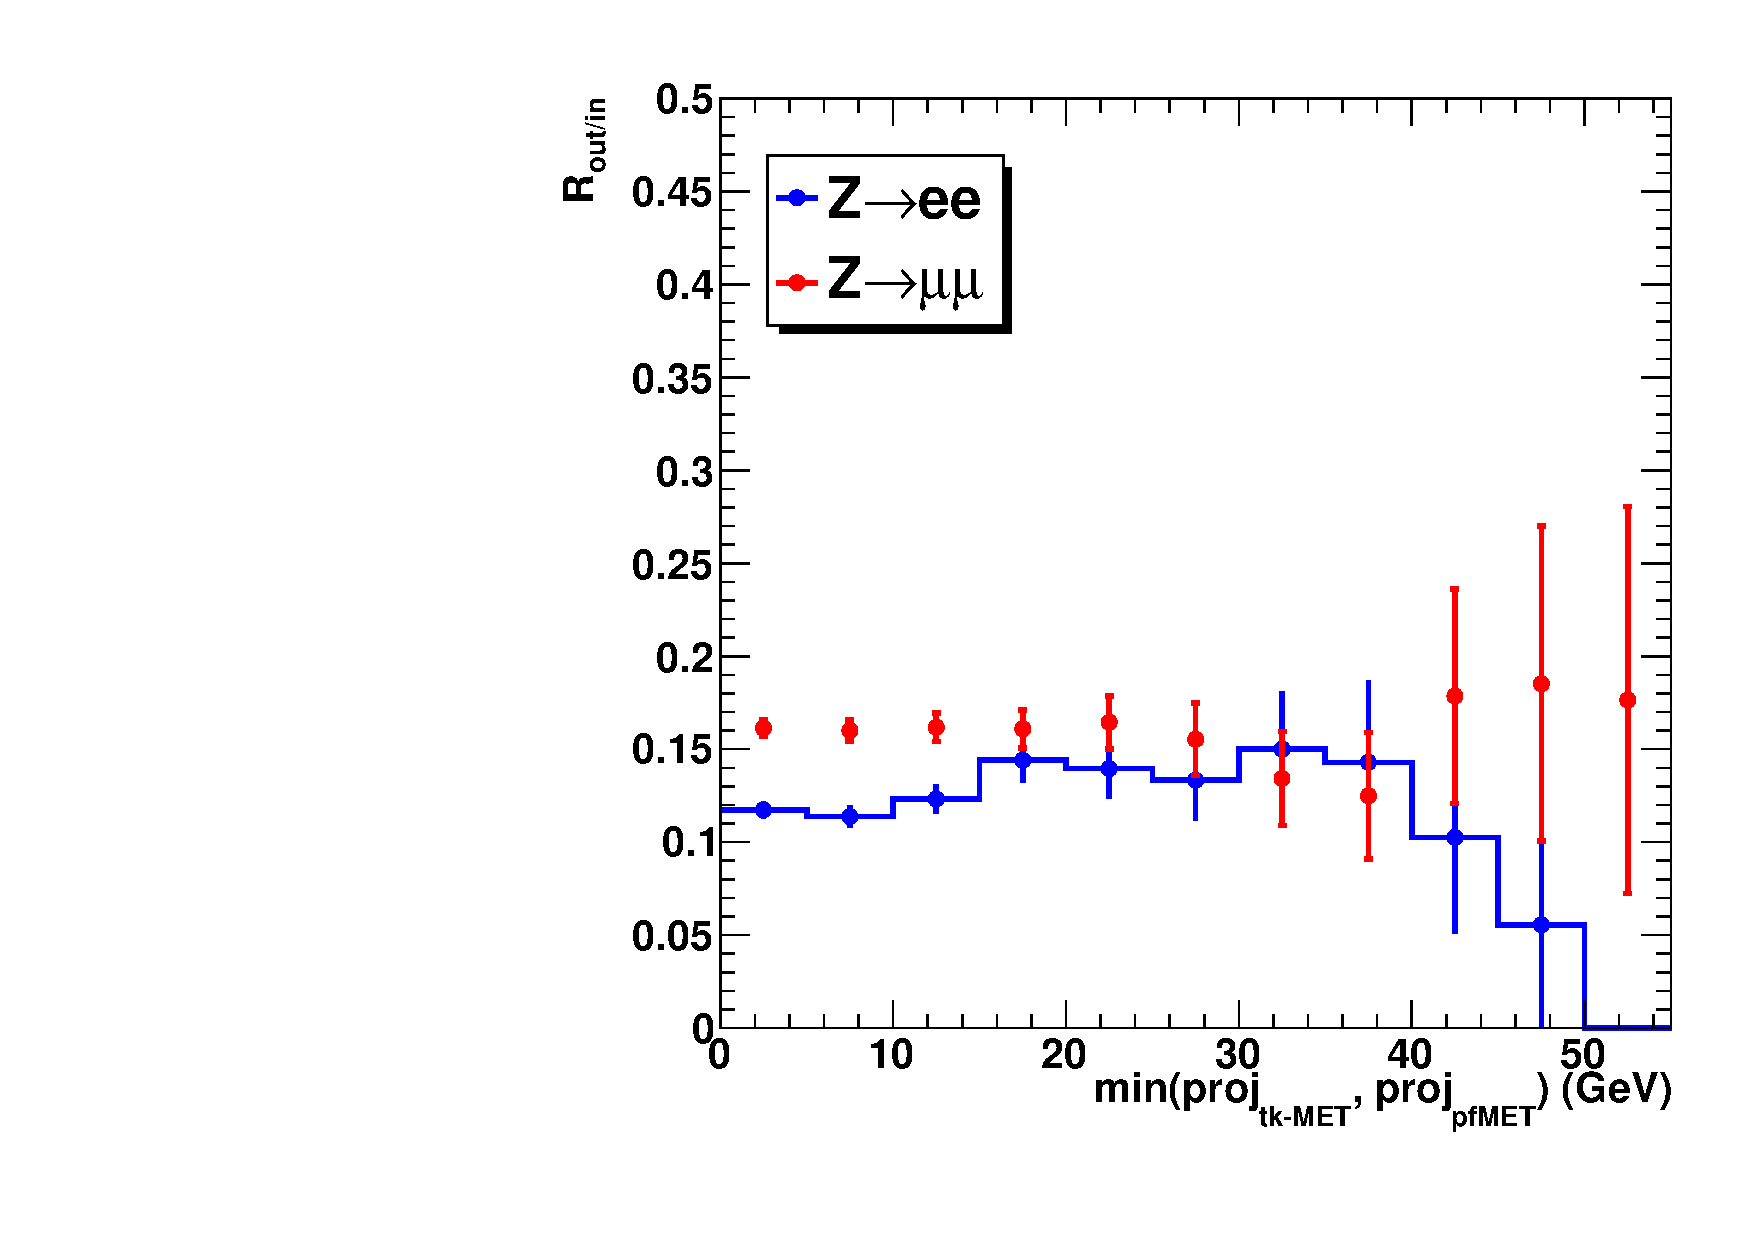
\includegraphics[width=0.3\textwidth]{figures/Routin_mc_2Jet.pdf}
%% \caption{ The ratio $R_{out/in}$ as a function of the $\met$ cut obtained using MC in the 
%% 0-Jet (left), 1-Jet (middle) and 2-Jet (right) bins. The event content in each 
%% bin is uncorrelated. The last bin represent the $R_{out/in}$ measured with min-MET $>$ 40 GeV. 
%% } %The difference in the ratio between 
%% %\ee\ and \mm\ final states is due to lower minimum muon momentum compared with electron
%% %(10 GeV vs 15 GeV), which allows for more low mass Drell-Yan events.}
%% \label{fig:routin_met}
%% \end{center}
%% \end{figure}
%% %%%%%%%%%%%%%%%%%%%%%%%%%%%%%%


%% We apply a data-driven method~\cite{dyestnote} to estimate the $\dyll$
%% contributions in the same flavor $\ell^+\ell^-$ final states. %This
%% %method also provides an estimate for the \emph{resonant component} of
%% %$WZ$ and $ZZ$ contributions, in which both leptons come from the same
%% %$Z$ boson.

%% The expected contributions from $\dyll$ events outside the $Z$-mass
%% region in data can be estimated by counting the number of events near
%% the $Z$ mass region in data, subtracting from it the non-$Z$
%% contributions, and scaling it by a ratio $R_{out/in}$ defined as the
%% fraction of events outside and inside the $Z$-mass region in the
%% simulation. The non-$Z$ contributions close to the $Z$-mass region in
%% data is estimated from the number of events in the $e^\pm\mu^\mp$
%% final state $N_{in}^{e\mu}$, applying a correction factor that
%% normalizes the electron-to-muon efficiency $k_{ee/\mu\mu}$. 
%% $R_{out/in}$ can be obtained both from simulation and
%% data.  In simulation it is defined as the ratio
%% $N_{out}^{MC}/N_{in}^{MC}$. 
%% %$N_{out}^{MC}/N_{in}^{MC}$ with a looser $\met$ cut of 20 GeV
%% %(referred to as a loose selection).  This method is described
%% This method is described mathematically in Eq.~\ref{eq:dyest}.
%% %%%%%%%%%%%%%%%%%%%%%%%%%%%%%%
%% \begin{eqnarray}
%% %N_{out}^{ll,exp} = R_{out/in}^{ll,loose}(N_{in}^{ll} - 0.5N_{in}^{e\mu}k_{ll}), 
%% N_{out}^{ll,exp} = R_{out/in}^{ll}(N_{in}^{ll} - 0.5N_{in}^{e\mu}k_{ll}), 
%% \label{eq:dyest}
%% \end{eqnarray}
%% %%%%%%%%%%%%%%%%%%%%%%%%%%%%%%
%% where $k_{ee} = \sqrt{\frac{N_{in}^{ee,loose}}{N_{in}^{\mu\mu,loose}}}$ for 
%% $\dyee$ and $k_{mm} = \sqrt{\frac{N_{in}^{\mu\mu,loose}}{N_{in}^{ee,loose}}}$ 
%% for $\dymm$. In the $k_{ll}$ calcualtion, we apply a loose $\met$ cut of 20 GeV. 
%% The values of $R_{out/in}$ as estimated from simulation are reported
%% in Table~\ref{tab:Routinmc} at the \ww\ preselection level. 

%% %%%%%%%%%%%%%%%%%%%%%%%%%%%%%%%
%% \begin{table}
%% \begin{center}
%% \begin{tabular}{c c c c }
%% \hline
%% \vspace{-3mm} && \\
%% Jet Bin & $R_{out/in}^{mm}$ &  $R_{out/in}^{ee}$  &   $R_{out/in}^{ee,mm}$\\
%% \vspace{-3mm} &&& \\
%% \hline
%% 0 & 0.23 $\pm$ 0.09 $\pm$ 0.10 & 0.29 $\pm$ 0.09 $\pm$ 0.11 & 0.25 $\pm$ 0.06 $\pm$ 0.05\\
%% 1 & 0.15 $\pm$ 0.04 $\pm$ 0.15 & 0.14 $\pm$ 0.03 $\pm$ 0.05 & 0.15 $\pm$ 0.03 $\pm$ 0.10\\
%% 2 & 0.16 $\pm$ 0.03 $\pm$ 0.13 & 0.13 $\pm$ 0.03 $\pm$ 0.06 & 0.15 $\pm$ 0.02 $\pm$ 0.10\\
%% \hline
%% \end{tabular}
%% \end{center}
%% \caption{The ratio $R_{out/in}^{ll}$ at different jet bins evaluated from MC, applying the min-MET $>$ 40 GeV selection.
%% \label{tab:Routinmc}}
%% \end{table}
%% %%%%%%%%%%%%%%%%%%%%%%%%%%%%%%


%% %%%%%%%%%%%%%%%%%%%%%%%%%%%%%%
%% \begin{figure}[!htbp]
%% \begin{center}
%% 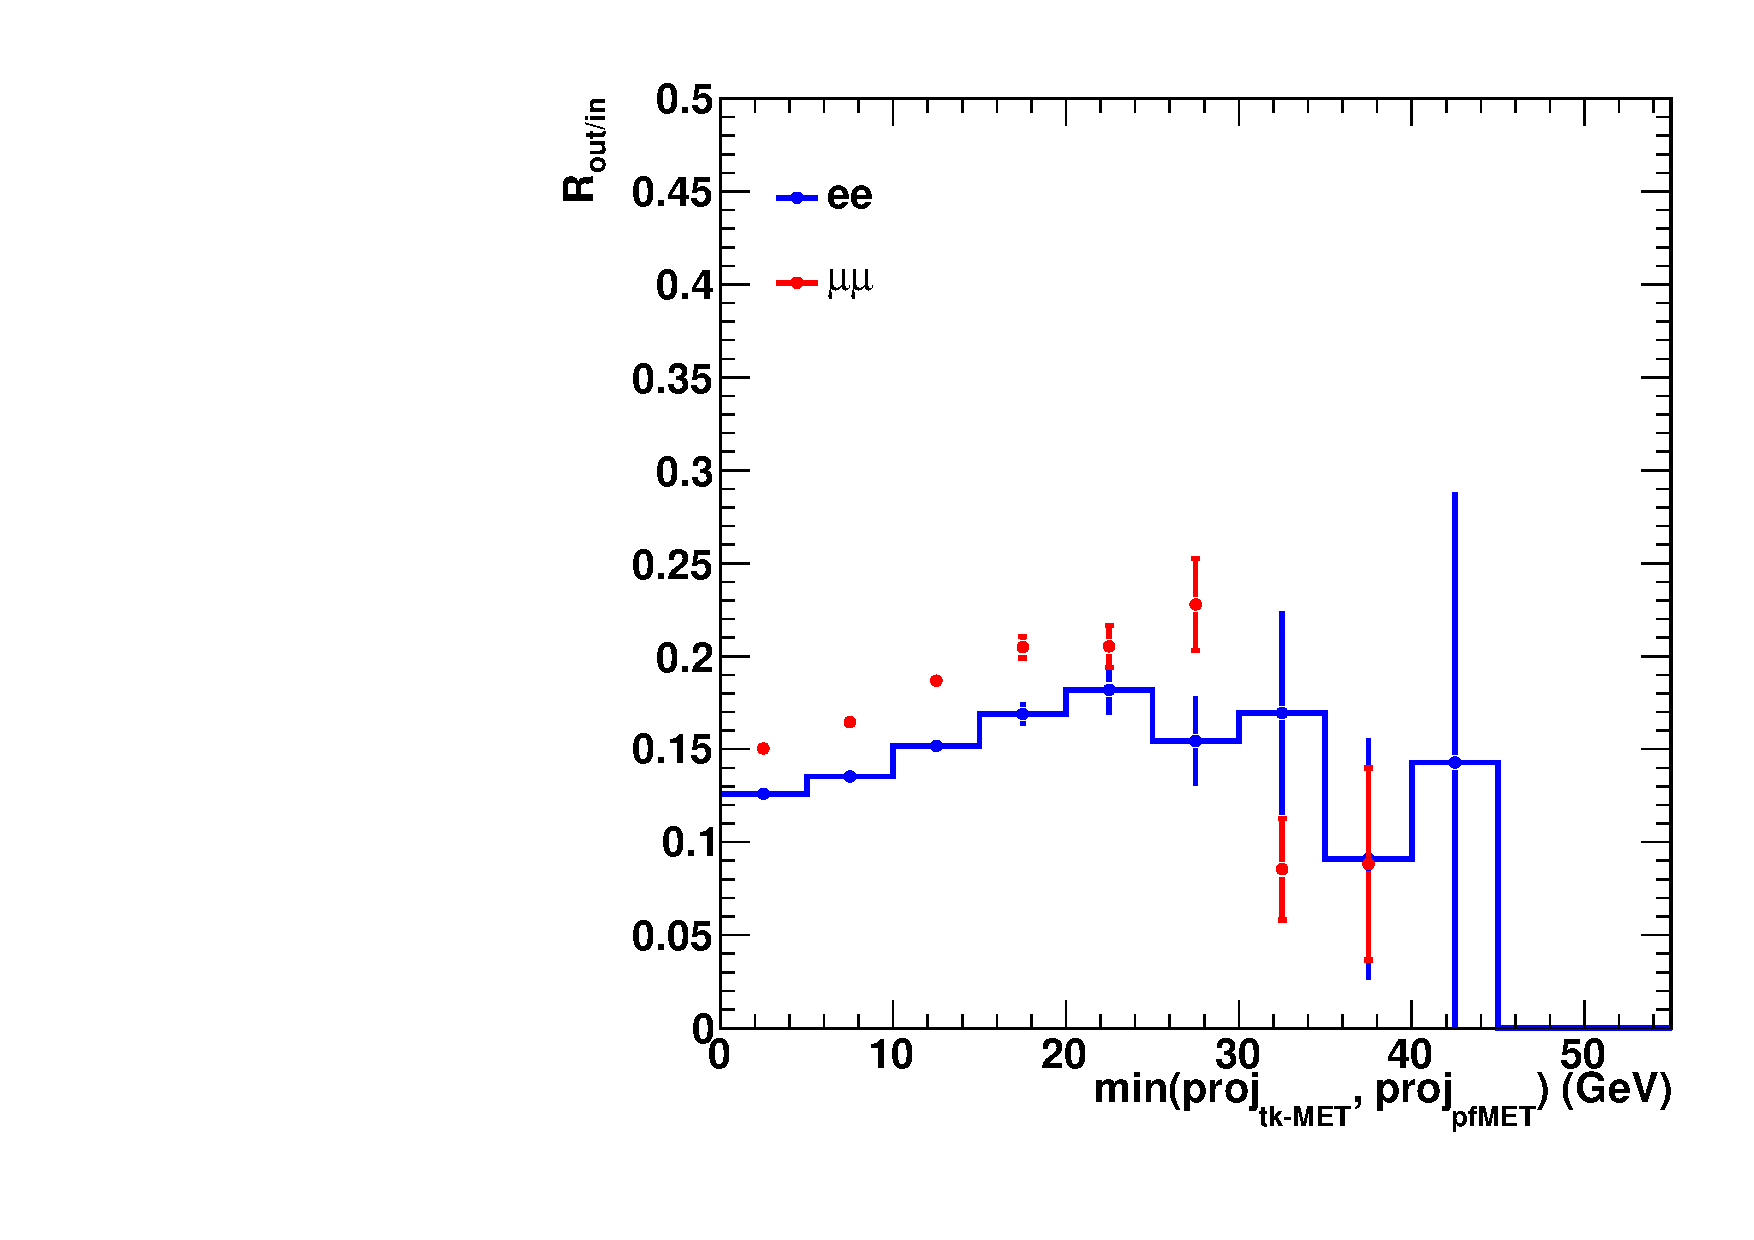
\includegraphics[width=0.3\textwidth]{figures/Routin_mc_0Jet.pdf}
%% 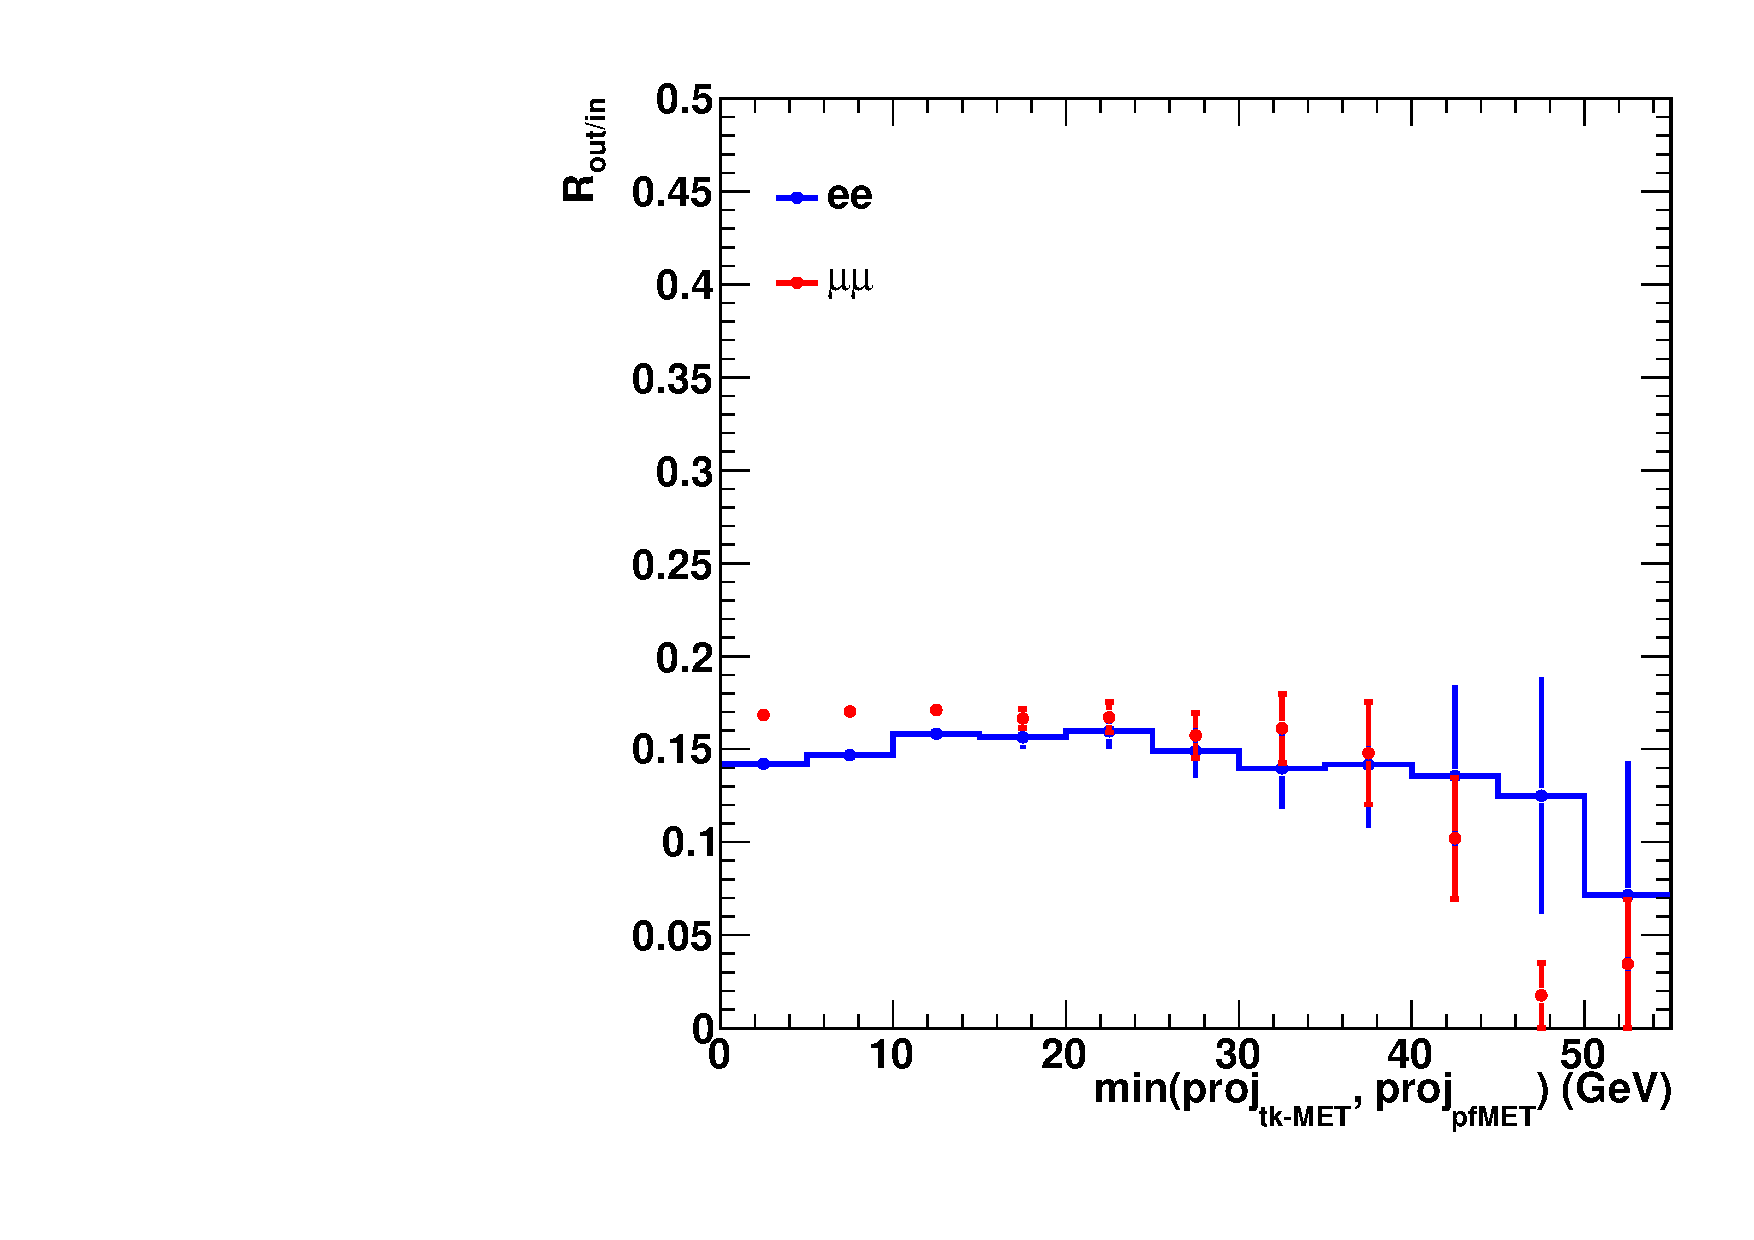
\includegraphics[width=0.3\textwidth]{figures/Routin_mc_1Jet.pdf}
%% 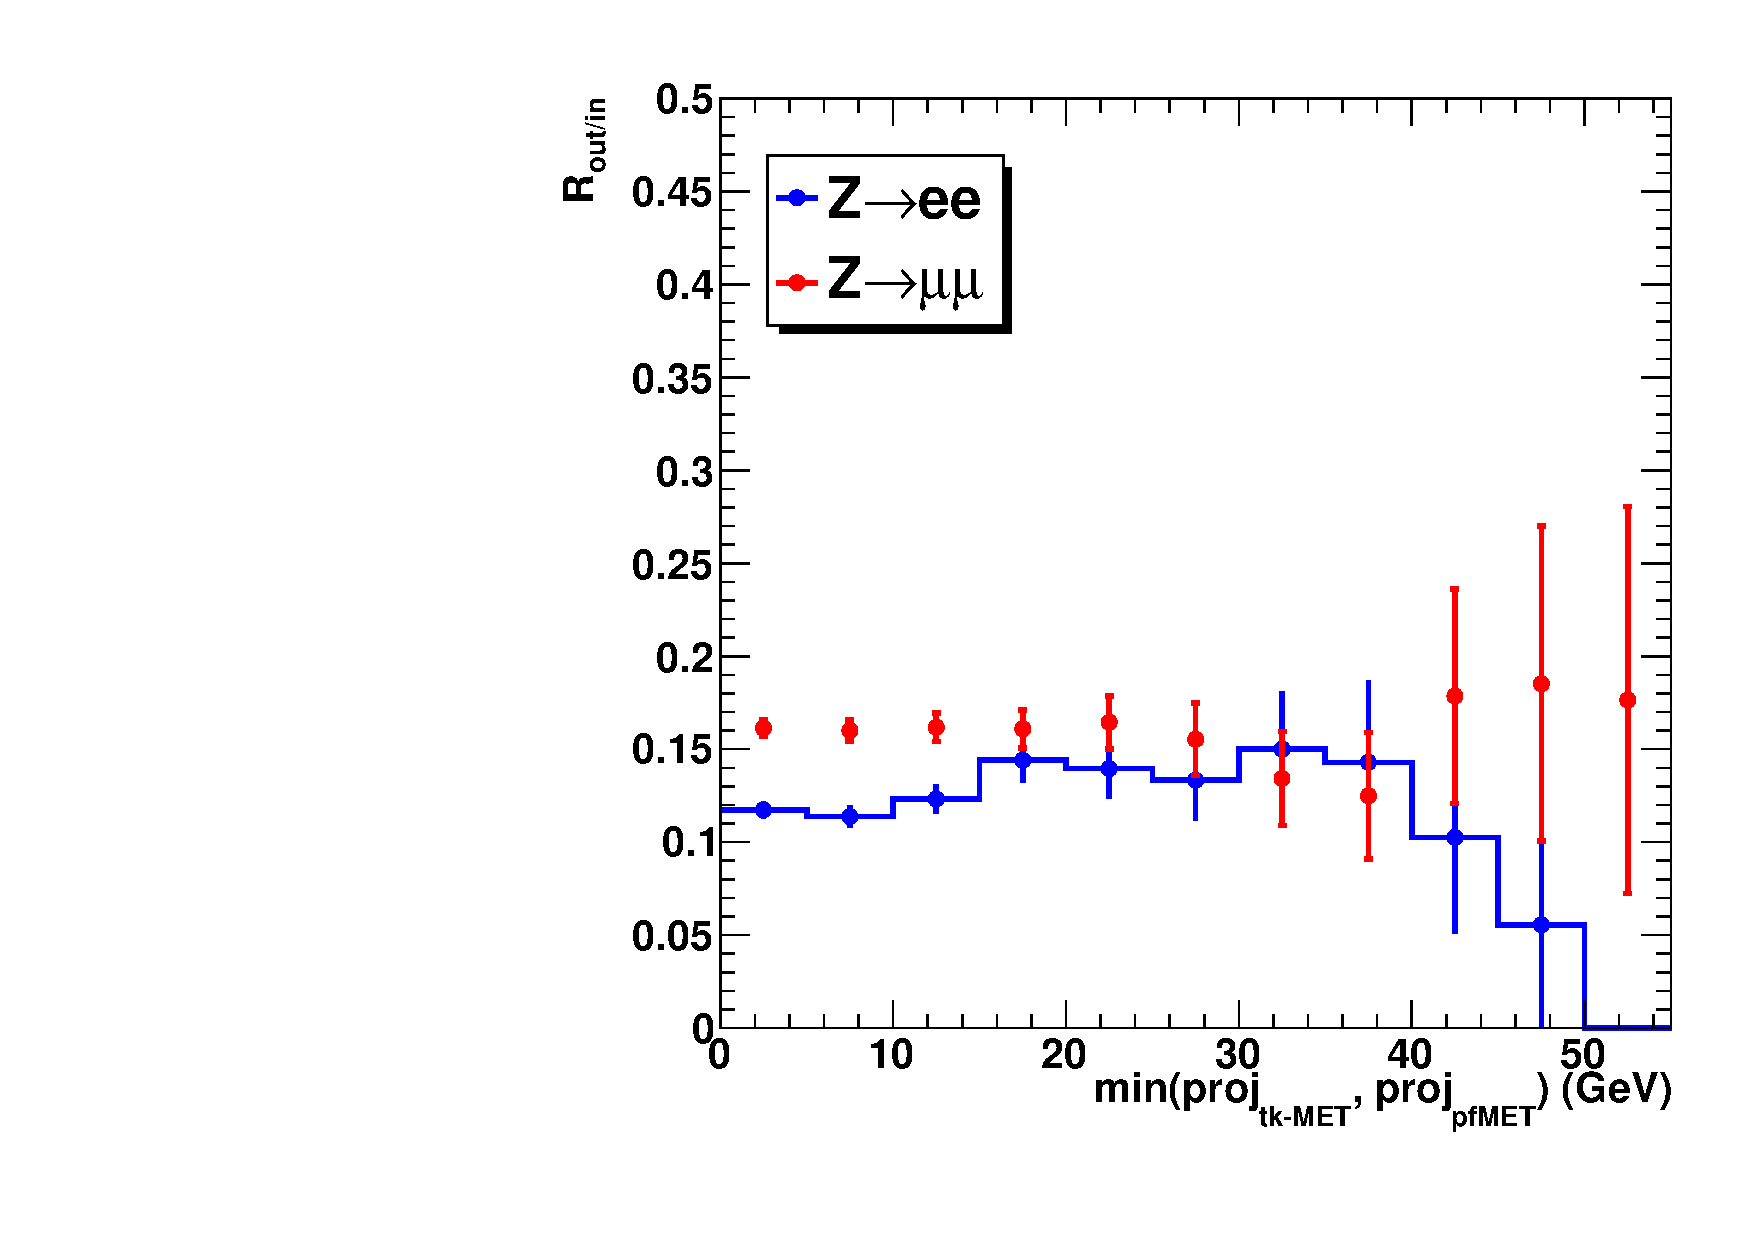
\includegraphics[width=0.3\textwidth]{figures/Routin_mc_2Jet.pdf}
%% \caption{ The ratio $R_{out/in}$ as a function of the $\met$ cut obtained using MC in the 
%% 0-Jet (left), 1-Jet (middle) and 2-Jet (right) bins. The event content in each 
%% bin is uncorrelated. The last bin represent the $R_{out/in}$ measured with min-MET $>$ 40 GeV. 
%% } %The difference in the ratio between 
%% %\ee\ and \mm\ final states is due to lower minimum muon momentum compared with electron
%% %(10 GeV vs 15 GeV), which allows for more low mass Drell-Yan events.}
%% \label{fig:routin_met}
%% \end{center}
%% \end{figure}
%% %%%%%%%%%%%%%%%%%%%%%%%%%%%%%%


%% %%%%%%%%%%%%%%%%%%%%%%%%%%%%%%
%% \begin{figure}[!htbp]
%% \begin{center}
%% 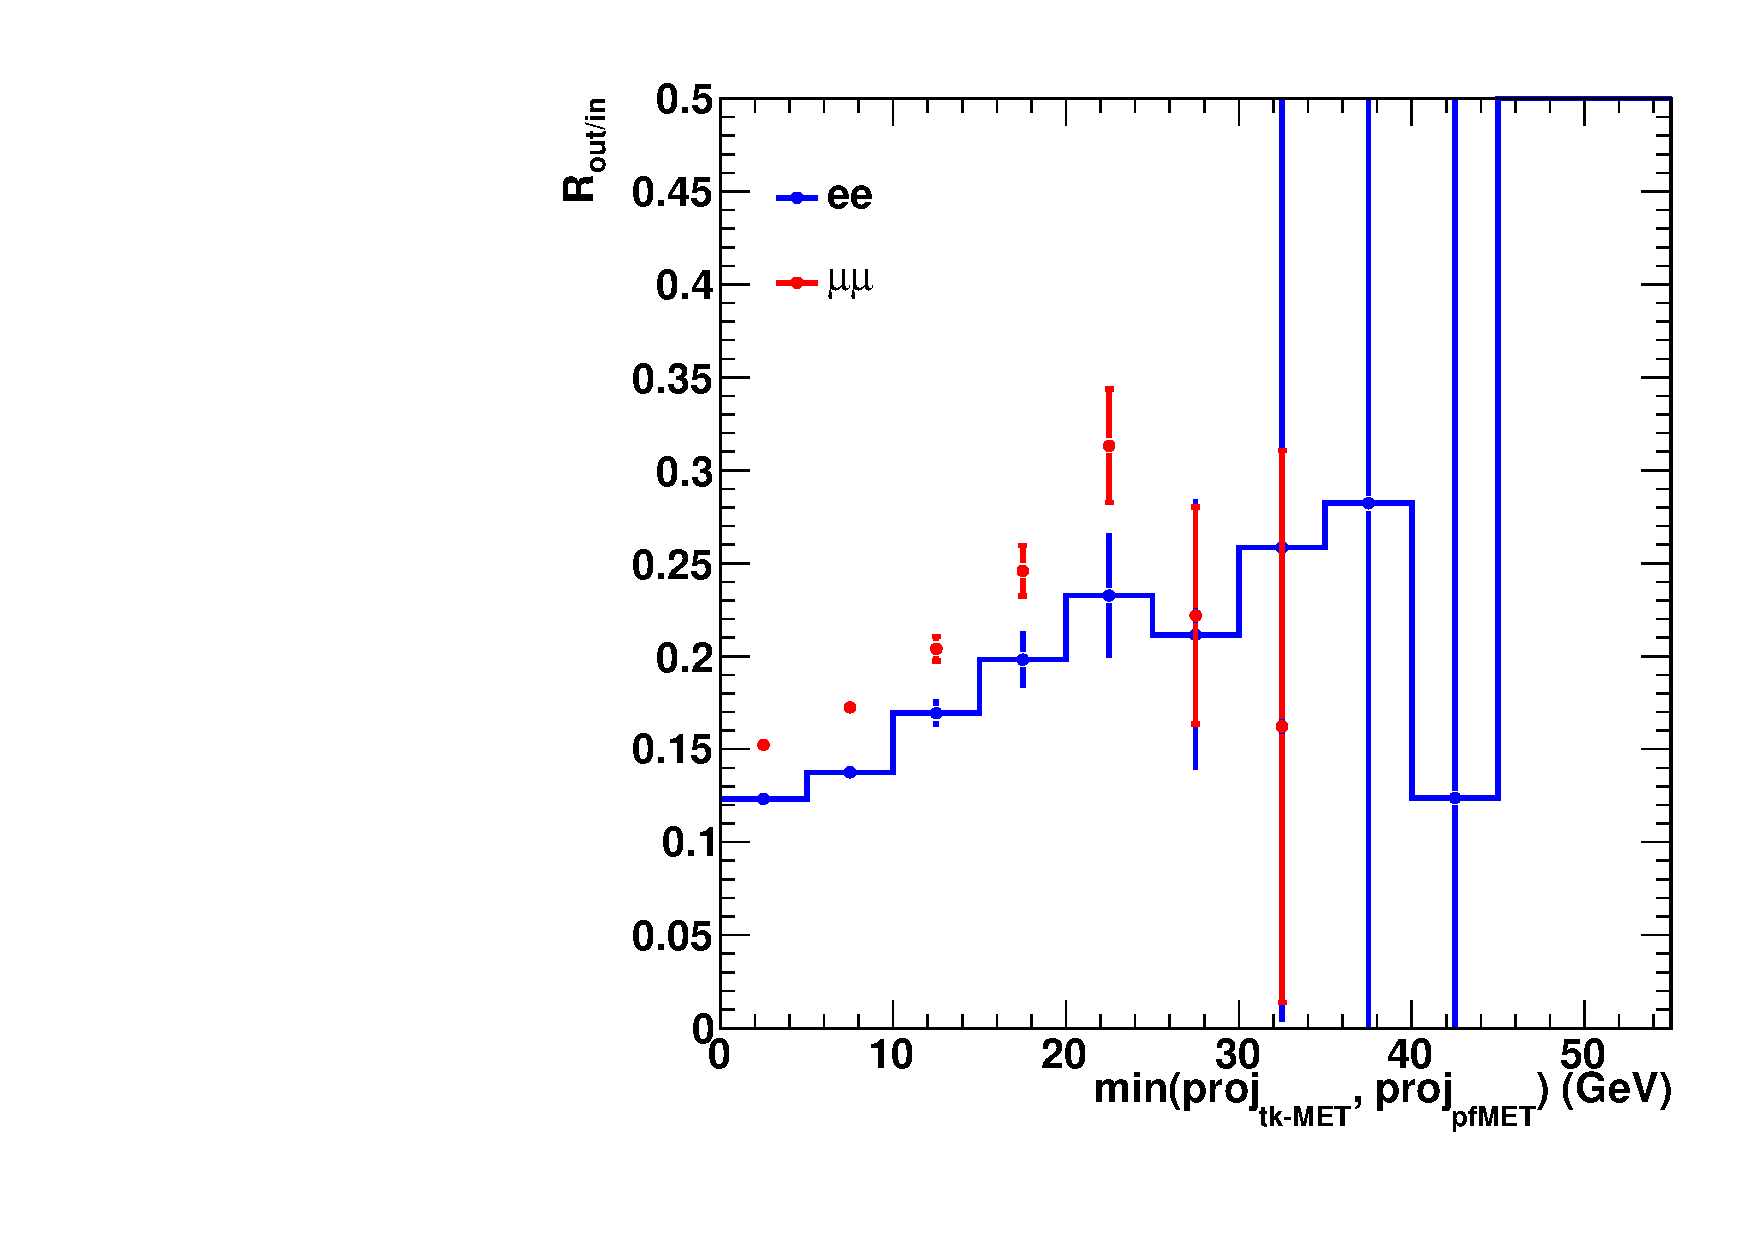
\includegraphics[width=0.3\textwidth]{figures/Routin_data_0Jet.pdf}
%% 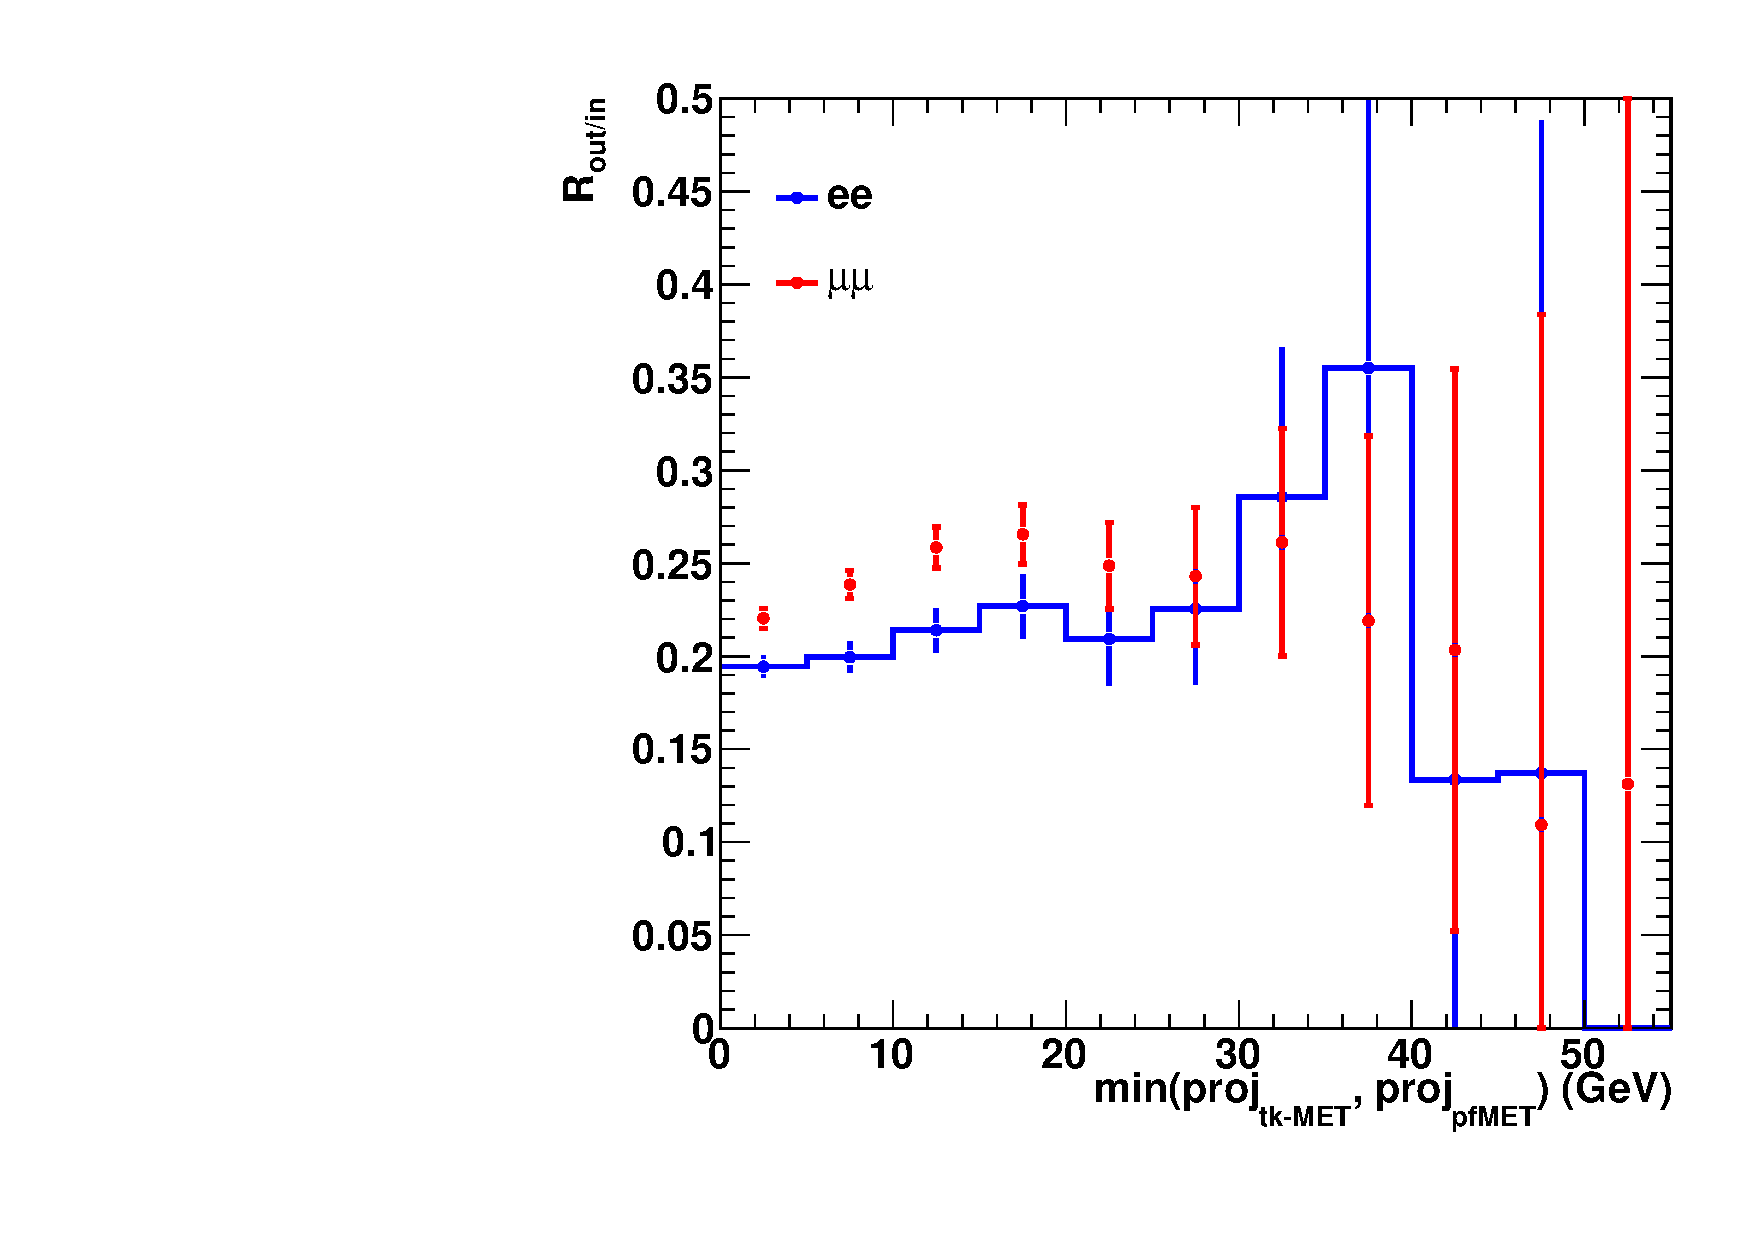
\includegraphics[width=0.3\textwidth]{figures/Routin_data_1Jet.pdf}
%% 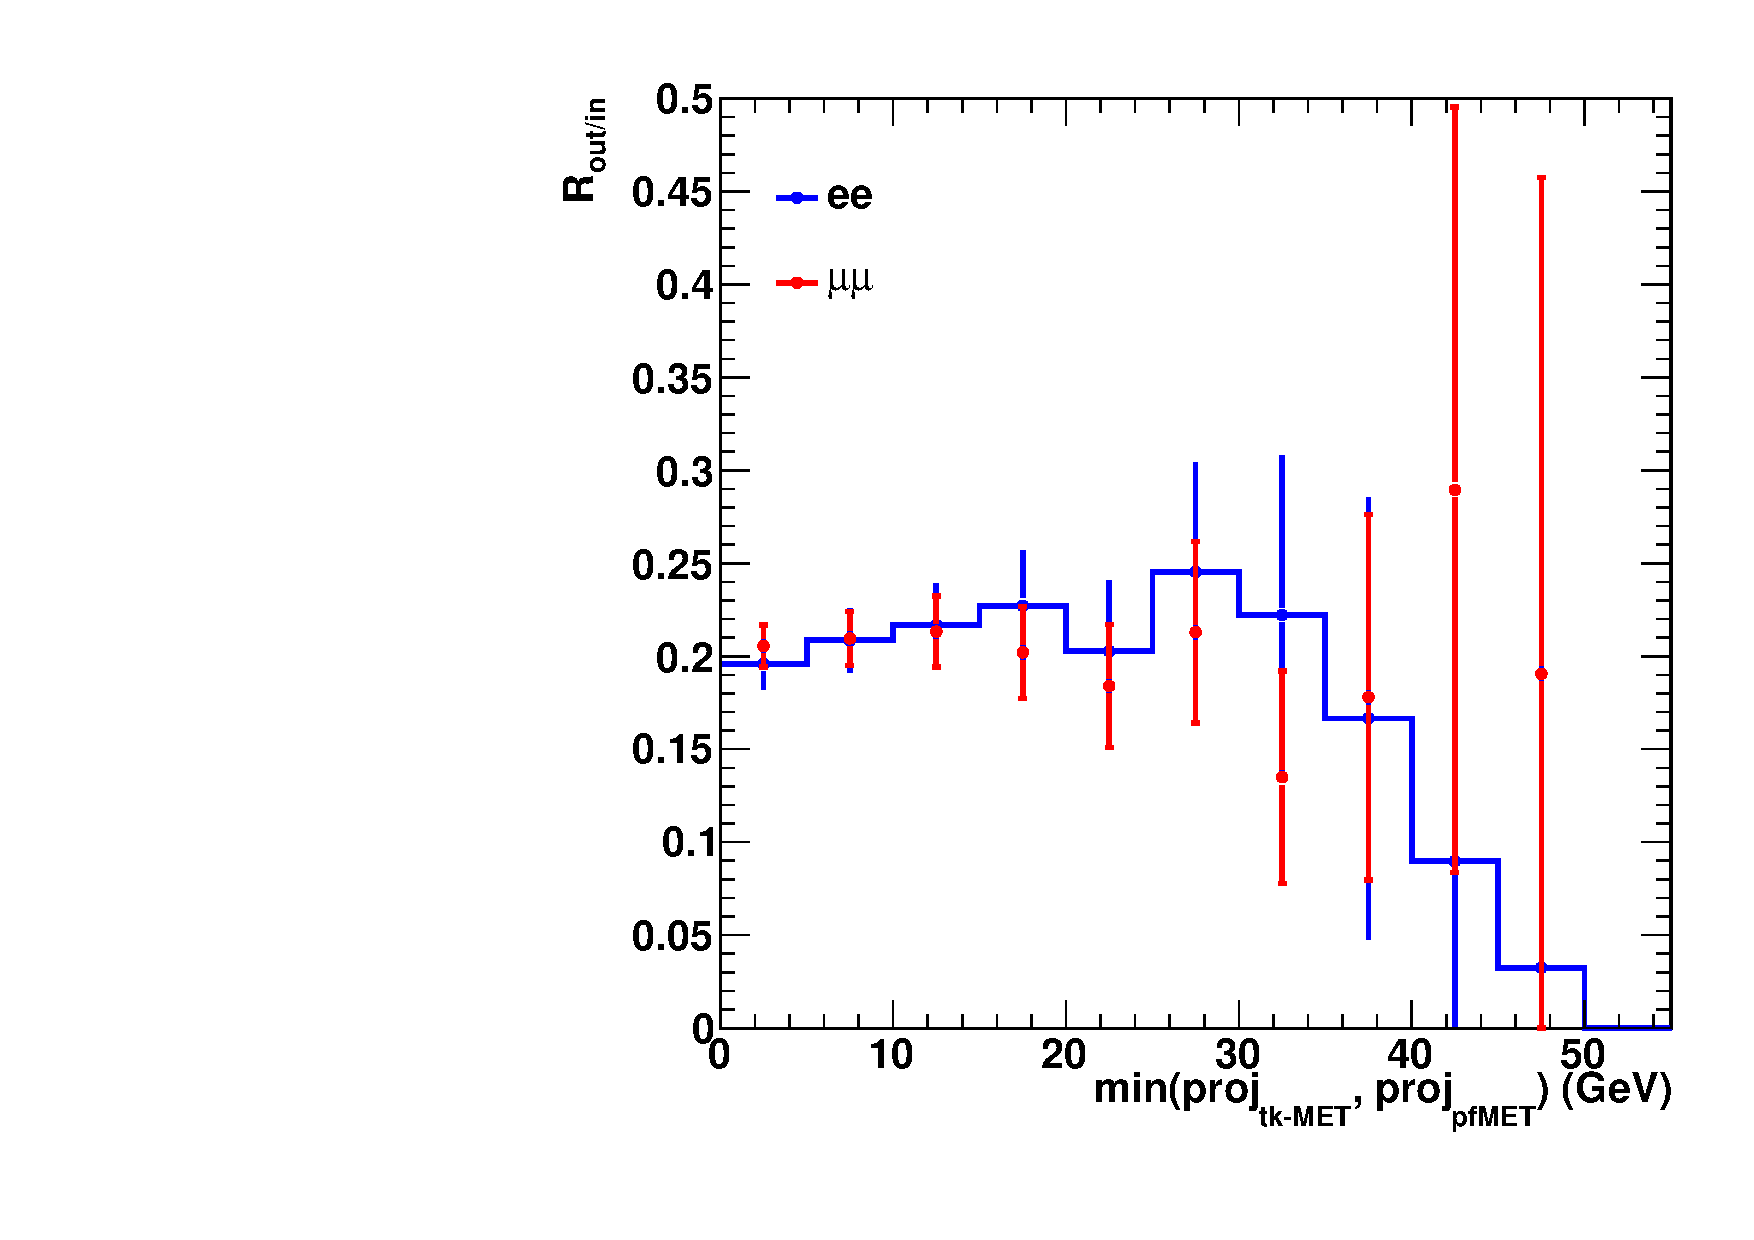
\includegraphics[width=0.3\textwidth]{figures/Routin_data_2Jet.pdf}
%% \caption{ The ratio $R_{out/in}$ as a function of the $\met$ cut obtained using data in the 
%% 0-Jet (left), 1-Jet (middle) and 2-Jet (right) bins. The event content in each 
%% bin is uncorrelated. The measurements are done only in the control region where min-MET $<$ 40 GeV, 
%% therefore the last bin is not filled. }
%% %The difference in the ratio between 
%% %\ee\ and \mm\ final states is due to lower minimum muon momentum compared with electron
%% %(10 GeV vs 15 GeV), which allows for more low mass Drell-Yan events.}
%% \label{fig:routin_met_data}
%% \end{center}
%% \end{figure}
%% %%%%%%%%%%%%%%%%%%%%%%%%%%%%%%


%% %% There are two ways in which the combination of DY and ZZ/ZW
%% %% backgrounds can be treated: one possibility is to use
%% %% equation \eqref{eq:dyest} for the combination of DY and peaking
%% %% ZZ/ZW background $(\textrm{Z} \to \ell\ell) +
%% %% (\textrm{W\!/Z} \to \textrm{any})$
%% %% %%%%%%%%
%% %% \begin{equation}\label{eq:dyExtrapM2}
%% %%   N(\ell\ell)_{\textrm{signal}} ^{\textrm{DY}+\textrm{ZV}} =
%% %%   (N(\ell\ell)_{\textrm{control}}^{\textrm{data}}-0.5\times
%% %%   N(e\mu)_{\textrm{control}} ^{\textrm{data}}\times k_{\ell\ell}
%% %%   ) \times R(\ell\ell)_{out/in}^{\textrm{DY}+\textrm{ZV}}
%% %% \end{equation}
%% %% %%%%%%%%%
%% %% and then add separately the non-peaking ZZ/ZW from simulation.  

%% The ZZ/ZW processes contribute to the events in the control region 
%% of the $m_{\ell\ell}$ region dominated by the DY. 
%% The contribution from ZZ/ZW becomes comparable to the Drell-Yan background 
%% after a tight projected \met selection of 40 GeV. 
%% The ZZ/ZW events contain natural \met, for which
%% the detector simulation is reliable\footnote{The ZZ/ZW events with
%% no \met are suppressed by the same large factor as the DY ones, and
%% therefore their contribution is as negligible at the level of the
%% final selection as it would be in the yield at the Z peak without \met
%% requirement.}. 
%% We subtract the expected peaking ZZ/ZW
%% contribution to the yield in the Z peak using the simulation in the 
%% estimation of number of events within the $Z$ window in data:
%% %The ZZ/ZW expectation is taken from simulation.
%% %the extrapolation from the subtracted yield, and then include the full
%% %ZZ/ZW expectation from simulation as a background of the analysis:
%% %%%%%%%%%%
%% \begin{equation}\label{eq:dyExtrapM3}
%%   N(\ell\ell)_{\textrm{signal}} ^{\textrm{DY}}=
%%   (N(\ell\ell)_{\textrm{control}}^{\textrm{data}}-0.5\times
%%   N(e\mu)_{\textrm{control}} ^{\textrm{data}}\times k_{\ell\ell}
%%   -N_{\textrm{control}}^{\textrm{ZV, sim.}} )  \times
%%   R(\ell\ell)_{out/in}^{DY}
%% \end{equation}
%% %%%%%%%%%%%%
%% %The subtraction using the simulation is legitimate since 
%% The ZZ/ZW contribution in the same flavor final states is then 
%% taken directly from simulation. 
%% Seperating the Drell-Yan and ZZ/WZ components 
%% accounts for the fact that the extrapolation from control 
%% region to signal region can be different for the two processes when
%% considering the full Higgs selection. We assume an overall 10\%
%% uncertainty on the ZZ/ZW yield in the peak, which is anyway
%% overshadowed by the statistical uncertainty on the observed events in
%% the Z peak in data.
%% % The second approach, that keeps the two components
%% %separate, This accounts for the fact that the extrapolation from control

%% The estimation from the on peak region relies on the assumption that
%% the dependence of the ratio $R_{out/in}$ on the $\met$ cut is well
%% modelled by the simulation and is relatively flat.
%% Figure~\ref{fig:routin_met} shows the ratios $R_{out/in}$ as functions
%% of the $\met$ cut at different jet bins determined from simulation at 
%% the \ww preselection level. The systematic uncertainty is assigned as the 
%% largest difference in the ratio to the central value as we vary the 
%% $\met$ cut from 0 to 40 GeV. 

%% We cross-checked the $R_{out/in}$ value in data.  Background processes
%% contribute equally to $ee$, $e\mu$, $\mu e$ and $\mu\mu$ final states
%% (after efficiency corrections), while Drell-Yan only contributes to
%% $ee$ and $\mu\mu$. Therefore we can subtract $e\mu$ and $\mu e$
%% contribtutions from $ee$ and $\mu\mu$ ones to get an estimate of
%% Drell-Yan.  Figure~\ref{fig:routin_met_data} shows the dependence of
%% $R_{out/in}$ of $\met$ cut evaluated in data.


%% %We then estimate the $R_{out/in}$ at a looser $\met$ selection
%% %($\met>$ 20 GeV) with respect the analysis one ($\met>$ 35 GeV).
%% %which allows not to run out of statistics in the $Z\to\ell\ell$ sample,
%% %both in case of simulation and data.

%% The value of $R_{out/in}$ changes as a function of the tight
%% kinematics requirements applied to select the Higgs signal region
%% (among which the tighter $\met$ cuts).  So we take the nominal value
%% from data estimation at the full Higgs selection, where no further
%% extrapolation is needed except the {\it in/out} region of the Z peak. 
%% To gain statistics, the $R_{out/in}$ is evaluated without applying the 
%% transverse mass cuts. 

%% We show the number of selected events in the Z peak region in data,
%% the correspondent value of $R_{out/in}$ and the comparison between the
%% expected DY contribution and the measured one in
%% Table~\ref{tab:routin_data_zeroj} and in Table~\ref{tab:routin_data_onej}
%% for zero and one jet bins, respectively. In the measurements we combine the 
%% $\zee$ and $\zmm$ contributions. 

%% %%%%%%%%%%%%%%%%%%%%%%%%%%%%%%
%% \begin{table}
%% \begin{center}
%% \begin{tabular}{c c c c c}
%% \hline
%% \vspace{-3mm} && \\
%% mass   & $N_{in}^{data}(DY)$ & $\langle R_{out/in} \rangle$ & $N_{out}^{data}(DY)$ & $N_{out}^{MC}(DY)$ \\
%% \vspace{-3mm} && \\
%% \hline
%% WW & 25.64 $\pm$ 13.24 & 0.25 $\pm$ 0.06 $\pm$ 0.05 & 6.46 $\pm$ 3.70 $\pm$ 1.16 & 2.00 $\pm$ 0.44 \\   
%% \hline
%% 120 GeV & 11.43 $\pm$ 6.33  & 0.28 $\pm$ 0.09 $\pm$ 0.76 & 3.24 $\pm$ 2.09 $\pm$ 8.71 & 0.81 $\pm$ 0.29 \\   
%% 130 GeV & 1.00 $\pm$ 4.07   & 0.73 $\pm$ 0.28 $\pm$ 1.08 & 0.73 $\pm$ 2.99 $\pm$ 1.08 & 0.93 $\pm$ 0.31 \\   
%% 140 GeV & 0.71 $\pm$ 3.93   & 0.59 $\pm$ 0.25 $\pm$ 0.63 & 0.42 $\pm$ 2.33 $\pm$ 0.44 & 0.56 $\pm$ 0.22 \\   
%% 150 GeV & 1.00 $\pm$ 4.32   & 0.40 $\pm$ 0.23 $\pm$ 0.27 & 0.40 $\pm$ 1.74 $\pm$ 0.27 & 0.25 $\pm$ 0.13 \\       
%% 160 GeV & 1.18 $\pm$ 2.02   & 1.00 $\pm$ 0.71 $\pm$ 0.64 & 1.18 $\pm$ 2.19 $\pm$ 0.76 & 0.25 $\pm$ 0.13 \\     
%% 170 GeV & 2.04 $\pm$ 2.67   & 1.00 $\pm$ 0.80 $\pm$ 0.70 & 2.04 $\pm$ 3.14 $\pm$ 1.43 & 0.19 $\pm$ 0.14 \\          
%% 180 GeV & 0.41 $\pm$ 3.21   & 0.57 $\pm$ 0.44 $\pm$ 0.16 & 0.24 $\pm$ 1.84 $\pm$ 0.07 & 0.12 $\pm$ 0.12 \\         
%% 190 GeV & 4.69 $\pm$ 4.65   & 0.33 $\pm$ 0.24 $\pm$ 0.23 & 1.56 $\pm$ 1.90 $\pm$ 1.08 & 0.12 $\pm$ 0.12 \\          
%% 200 GeV & 4.25 $\pm$ 5.40   & 0.14 $\pm$ 0.09 $\pm$ 0.08 & 0.59 $\pm$ 0.84  $\pm$ 0.34 & 0.12 $\pm$ 0.12 \\             
%% 250 GeV & 2.09 $\pm$ 6.52   & 0.03 $\pm$ 0.02 $\pm$ 0.02 & 0.06 $\pm$ 0.20 $\pm$ 0.03 & 0.06 $\pm$ 0.06 \\          
%% 300 GeV & 0.57 $\pm$ 4.56   & 0.05 $\pm$ 0.05 $\pm$ 0.39 & 0.03 $\pm$ 0.23 $\pm$ 0.22 & 0.06 $\pm$ 0.06 \\
%% \hline
%% \end{tabular}
%% \caption{The Drell-Yan estimation in the same flavor final state in the zero-jet bin.
%% \label{tab:routin_data_zeroj}}
%% \end{center}
%% \end{table}
%% %%%%%%%%%%%%%%%%%%%%%%%%%%%%%%



%% %%%%%%%%%%%%%%%%%%%%%%%%%%%%%%
%% \begin{table}
%% \begin{center}
%% \begin{tabular}{c c c c c}
%% \hline
%% \vspace{-3mm} && \\
%% mass   & $N_{in}^{data}(DY)$ & $\langle R_{out/in} \rangle$ & $N_{out}^{data}(DY)$ & $N_{out}^{MC}(DY)$ \\
%% \vspace{-3mm} && \\
%% \hline
%% WW & 50.73 $\pm$ 10.69 & 0.15 $\pm$ 0.03 $\pm$ 0.10 & 7.39 $\pm$ 2.08 $\pm$ 5.11 & 3.24 $\pm$ 0.56 \\
%% \hline
%% 120 & 14.21 $\pm$ 4.01 & 0.07 $\pm$ 0.02 $\pm$ 0.23 & 0.96 $\pm$ 0.39 $\pm$ 3.24 & 0.87 $\pm$ 0.29 \\
%% 130 & 4.02 $\pm$ 2.66  & 0.13 $\pm$ 0.03 $\pm$ 0.41 & 0.51 $\pm$ 0.37 $\pm$ 1.64 & 1.06 $\pm$ 0.32 \\
%% 140 & 3.82 $\pm$ 2.66  & 0.11 $\pm$ 0.03 $\pm$ 0.26 & 0.43 $\pm$ 0.33 $\pm$ 1.00 & 1.06 $\pm$ 0.31 \\
%% 150 & 12.45 $\pm$ 4.26 & 0.08 $\pm$ 0.03 $\pm$ 0.15 & 0.94 $\pm$ 0.47 $\pm$ 1.90 & 0.56 $\pm$ 0.21 \\
%% 160 & 3.27 $\pm$ 3.20  & 0.23 $\pm$ 0.09 $\pm$ 0.32 & 0.75 $\pm$ 0.79 $\pm$ 1.03 & 0.56 $\pm$ 0.21 \\
%% 170 & 4.23 $\pm$ 3.35  & 0.23 $\pm$ 0.09 $\pm$ 0.22 & 0.97 $\pm$ 0.86 $\pm$ 0.92 & 0.37 $\pm$ 0.18 \\
%% 180 & 2.88 $\pm$ 3.51  & 0.18 $\pm$ 0.07 $\pm$ 0.10 & 0.52 $\pm$ 0.66 $\pm$ 0.28 & 0.31 $\pm$ 0.16 \\
%% 190 & 11.37 $\pm$ 4.73 & 0.08 $\pm$ 0.03 $\pm$ 0.13 & 0.94 $\pm$ 0.51 $\pm$ 1.47 & 0.44 $\pm$ 0.21 \\
%% 200 & 17.17 $\pm$ 5.61 & 0.07 $\pm$ 0.02 $\pm$ 0.08 & 1.15 $\pm$ 0.55 $\pm$ 1.36 & 0.44 $\pm$ 0.21 \\
%% 250 & 23.42 $\pm$ 6.39 & 0.07 $\pm$ 0.02 $\pm$ 0.01 & 1.67 $\pm$ 0.70 $\pm$ 0.31 & 0.75 $\pm$ 0.28 \\
%% 300 & 17.66 $\pm$ 5.04 & 0.05 $\pm$ 0.02 $\pm$ 0.07 & 0.90 $\pm$ 0.51 $\pm$ 1.30 & 0.37 $\pm$ 0.20 \\     
%% \hline
%% \end{tabular}
%% \caption{The Drell-Yan estimation in the same flavor final state in the one-jet bin.
%% \label{tab:routin_data_onej}}
%% \end{center}
%% \end{table}
%% %%%%%%%%%%%%%%%%%%%%%%%%%%%%%%

%% The method to estimate the Drell-Yan background performed for each
%% Higgs mass point is the most robust because it allows to do the
%% estimation directly on the signal kinematics region through a proper
%% estimation of $R_{out/in}$.  It leads to fairly large uncertainties on
%% the background mostly dominated by small event count in the Z-peak
%% area (see Appendix~\ref{app:dy_writeup}). It does not affect the mass points where we have sensitivity to
%% the Standard Model Higgs with current amount of data. 
%% With more data the uncertainties on the background estimation should improve.

